\documentclass[10pt]{book}
\usepackage{mathtools}
\usepackage{graphicx}
\usepackage[utf8]{inputenc}
\usepackage{float}
\usepackage{tabularx}
\usepackage{chngpage}
\usepackage{amsthm}
\usepackage{mathtools}
\usepackage{amsfonts}
\usepackage{tikz}
\usepackage{amssymb}
\usepackage{gensymb}
\usepackage{wrapfig}
\usepackage{enumerate}
\usepackage{braket}
\usepackage{pgfplots}
\usepackage{bbm}
\usepackage{fancyhdr}
\usepackage{emptypage}


%\numberwithin{equation}{section}
\newcommand{\R}{\mathbb{R}}
\newcommand{\F}{\mathcal{F}}
\renewcommand{\L}{\mathcal{L}}
\newcommand{\C}{\mathbb{C}}
\renewcommand{\H}{\mathcal{H}}
\newcommand{\Sum}{\sum_{n=0}^\infty}
\newcommand{\Res}[1]{\text{Res}f(z)\Big|_{#1}}
\newcommand{\vettore}[1]{\overrightarrow{#1}}
\newcommand{\p}{\mathbf{p}}
\newcommand{\x}{\mathbf{x}}
\renewcommand{\r}{\mathbf{r}}


\usepackage[a4paper, inner=1.5cm, outer=3cm, top=3cm, 
bottom=3cm, bindingoffset=1cm,headheight=110pt]{geometry} 


\pagestyle{fancy}
\fancyhf{}
\fancyhead[LE]{\leftmark}
\fancyhead[RO]{\rightmark}
\fancyfoot[C]{\thepage}
\begin{document}
\begin{titlepage}
  \pagestyle{empty}

  \begin{center}
    {\bfseries
      \Large {\huge U}NIVERSITY OF {\huge T}RENTO}

    \vspace{0.2cm}

    {\Large Department of Physics}

    \vspace{0.5cm}

    \begin{center}
      
\includegraphics[width=0.3\textwidth]{img/logo_unitn.png}
    \end{center}

    \vspace{0.5cm}

    {\bfseries \Large Degree course in Physics}

    \vspace{0.3cm}
    \line(1,0){338}
    \vspace{0.3cm}

    {\Large Final Thesis}

    \vspace{2.5cm}

    {\huge \textsc{Generation and manipulation of}}

    \vspace{0.4cm}

    {\huge \textsc{entangled photon pairs in}}

     \vspace{0.4cm}

     {\huge \textsc{coupled resonators}}
    

    \vspace{3.0cm}


    \large
    \begin{center}
      \begin{tabular}{ccc}
        {\bfseries Supervisor} &
        \hspace{5cm}
        {\bfseries Candidate} \\

        Prof. Lorenzo Pavesi &
        \hspace{5cm} Marco Canteri \\


      \end{tabular}
    \end{center}
    \vspace{2cm}

    {\bfseries \large Academic year 2016-2017}
    \vfill
  \end{center}
\end{titlepage}

\tableofcontents
\chapter{Introduction}
The aim of this thesis is to describe a theoretical model for the generation of entangled photons inside silicon optic chips. In particular, the structure i'm going to study is composed by two microrings side coupled to two channel waveguide. The geration of entangled photons is obtained exploiting non linear proprieties of silicon. In order to fullfil this goal, the second chapter gives a description of the needed basic structures, the microrings and the waveguides and how we can describe their behaviour using a mathematical formalism. The third chapter is devoted to the explanation of the physics behind the phenomena and the mathematics which can be used to carry out the calculation. Finally in the fourth chapter the model and the results are presented. The rest of the introduction is an overview on photonics. 
\section{Integrated optics}
The microelectronic has been widely succesfull and it was a revolution that has changed our daily life and works, nowdays microelectronics is present almost everywhere. The great success of this technologies is due to many reasons, one of them is the computational power of a small chip which for the Moore's law is predicted to be doubled every to years. The prediction still holds today, but we are reaching saturation point, in fact the improvements were possible by increasing the clock frequencies of the processing units, this kind of improvement faces several problems, such as heating power, antenna effects and RC time delays. Therefore, in order to keep the improvements going, the approch used is now to increase the number of processing units, but the problems are still present, they are only changed. The cores needs to communivate among them, so the problem is to realize efficient communication with high bandwidth and low power consumption. Photonics is a platform that can be used to achive such goal, with light is possible to realize ultra-high speed switch, it has low power consumption and it doesn't have electromagnetic noise. Several platform has been developed with different media, for example silicon, lithium niobate, arsenium gallium compounds. Since the electronics industry is based on silicon, Silicon-on-Insulator photonics is a promising platform to build optical chip. The technologies used for the fabrication of silicon chip is well studied and understood, it reached a high maturation and the industry and the infrastructure already exist. Futhermore silicon photonics has the compatiblity with the CMOS technlogy used is electronic chip, hence hybrid chip with electronics and photonics can be realised. Another important feature of silicon is the transparency at the important Telecom wavelenghts 1300-1600 nm, which allows the fabrications of photonic circuit with very low power loss. The aim of silicon photonics is to follow the philosophy behind microelectronics, small chip composed by few building block that can be used to build different devices changing the topology if the chip, and to realize this building block with fewer materials as possible and with a standard among the manifacturies.\\
In quantum mechanics light has been quantized and the single particle, photon, has quantum proprietis.




\\
A silicon optic chip is realised with three different layers as depicted in figure \eqref{SOIstructure}, at the bottom we can find the substrate, a silicon layer which provides a base and a stable structure for the chip, just above it there is a layer made of silicon dioxide called cladding and finally at the top there is another silicon layer called core. The thickness of the substrate and the cladding is in the order of some $\mu m$, while the core has an height in the order of few hundreds $nm$. The refractive index of silicon is $n_{Si} \simeq 3.5$ in the range of the Telecom wavelenghts, while the refractive index of silicon dioxide is $n_{SiO_2}\simeq 1.54$ in the same range, this allows the confinement of light in the core layer by total internal refraction. Exactly like in optical fiber the light travelling in the core layer when reaches the boundaries with the layer underneath or with the air (refractive index $\simeq 1$) is reflected back if the angle of incidence is greater then a critical angle. 
\begin{figure}
\centering
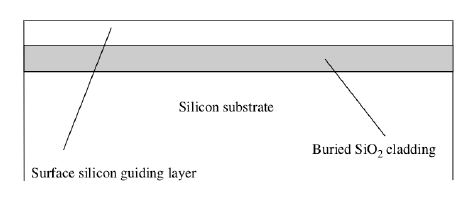
\includegraphics[width = .7\textwidth]{img/SOIstructure}
\caption{SOI chip layer structure}
\label{SOIstructure}
\end{figure}
\chapter{Silicon photonics building blocks}

\chapter{Formalism}

\section{Calculus}
The non linear Hamiltonian is
\[H_{NL} = -\frac{1}{3\varepsilon_0}\int\Gamma^{ijkl}_3(\r)D^iD^jD^kD^l\,d\r\]
where the summation over repeated indexes is implicit. A natural choice is to write the displacement operator associated with with channel $A$ in terms of the asymptotic-in fields, and the operator for channel $B$ and $C$ in terms of the asymptotic-out fields. So we can write the displacement operator as:
\[\mathbf{D}(\r) = \int_0^{+\infty}dk\sqrt{\frac{\hbar\omega_k}{2}}\left[a_{a,k}\mathbf{D}^{asy-in}_{a,k}(\r)+b_{b,k}\mathbf{D}^{asy-out}_{b,k}(\r)+b_{c,k}\mathbf{D}^{asy-out}_{c,k}(\r)\right] +\text{h.c.}\]
putting this inside expression () and keeping only the energy-conserving terms we arrive at:
\begin{equation}H_{NL} = -\int dk_1dk_2dk_3dk_4S_{bb}(k_1,k_2,k_3,k_4)a_{a,k_1}a_{a,k_2}b_{b,k_3}^\dagger b_{b,k_4}^\dagger -2\int dk_1dk_2dk_3dk_4S_{bc}(k_1,k_2,k_3,k_4)a_{a,k_1}a_{a,k_2}b_{b,k_3}^\dagger b_{c,k_4}^\dagger -\int dk_1dk_2dk_3dk_4S_{cc}(k_1,k_2,k_3,k_4)a_{a,k_1}a_{a,k_2}b_{c,k_3}^\dagger b_{c,k_4}^\dagger +\text{h.c.}\end{equation}
where we defined the following quantity
\[\hspace*{-1.2cm}S_{xy}(k_1,k_2,k_3,k_4) = \frac{3}{2\varepsilon_0}\sqrt{\frac{(\hbar\omega_{k_1})(\hbar\omega_{k_2})(\hbar\omega_{k_3})(\hbar\omega_{k_4})}{16}}\int d\r \Gamma^{ijkl}_3D^{i,asy-in}_{a,k_1}(\r)D^{j,asy-in}_{a,k_2}(\r)\left[D^{k,asy-out}_{x,k_3}(\r)\right]^*\left[D^{l,asy-out}_{y,k_4}(\r)\right]^* \]
with this expression in hands we can switch to the Heisenberg picture e we can define
\[V(t) = U_L^\dagger H_{NL}U_{L}\]
since the operator $U_L$ satisfies the unitary relation $U_L U_L^\dagger = U_L^\dagger U_L = \mathbbm{1}$ we can isert $U_L^\dagger U_L$ between every annhilation and creation operators and define the time dependent operators, for example $a_{k}(t) \equiv U_L^\dagger a_{k}U_L$. Time dependent operators satisfies the Heisenberg equation
\[\frac{da_{k}}{dt} = \frac{1}{i\hbar}[a_{k},H_L]\]
which we can solve for every operators. For example for $a_{k}$ the commutator with the linear Hamiltonian is:
\[[a_{k},H_L] = \int dk'\hbar \omega_{k'}a_{k} a_{k'}^\dagger a_{k'}-\int dk'\hbar \omega_{k'}a_{k'}^\dagger a_{k'}a_{k}\]
we know that $[a_k,a_{k'}^\dagger] = \delta(k-k')\implies a_{k} a_{k'}^\dagger = \delta(k-k') + a_{k'}^\dagger a_{k}$ substituting this into the first term we arrive at
\[[a_{k},H_L] = \int dk'\hbar \omega_{k'}a_{k}\delta(k-k') = \hbar \omega_{k}a_{k}\]
so the Heisenberg equation can be written as
\[\frac{da_{k}}{dt} = -i\omega_{k}a_{k}\]
which has the trivial solution $a_k(t) = a_k(0)e^{-i\omega_k t}$, since $a_k(0) = a_k$ we can write () as
\[V(t) \equiv = V_{bb} + 2V_{bc} + V_{cc}=\]
\end{document} 
